\section{Experimentos y resultados}

\subsection{Introducci\'on}
\begin{frame}
\frametitle{Experimentos}

\begin{table}[]
\centering
\scalebox{0.8}{
\begin{tabular}{cccc}
\hline
\textbf{No. de Sujeto}	
&   \textbf{Tiempo de Uso (Hr:Min)}		
&	\textbf{N\'umero de Nodos}
&   \textbf{Repeticiones} 	\\   
\hline

1				
&	166:23 						
&	1,494,792			
&	46,036				\\
		
2
&	490:24
&	1,333,016
&	116,001				\\
		
3
&	1060:48
&	1,448,016
&	378,541				\\
		
4
&	148:23
&	972,828
&	56,606				\\ 

5	
&	17:56
&	281,794
&	8,945				\\

6
&	285:45
&	1,570,951
&	130,220				\\

7	
&	37:40
&	418,966
&	23,660				\\
\hline

\end{tabular}
}
\caption{Informaci\'on de los datos recabados.}
\label{infodata}
\end{table}

\end{frame}

\begin{frame}
\begin{figure}[h]
\centering
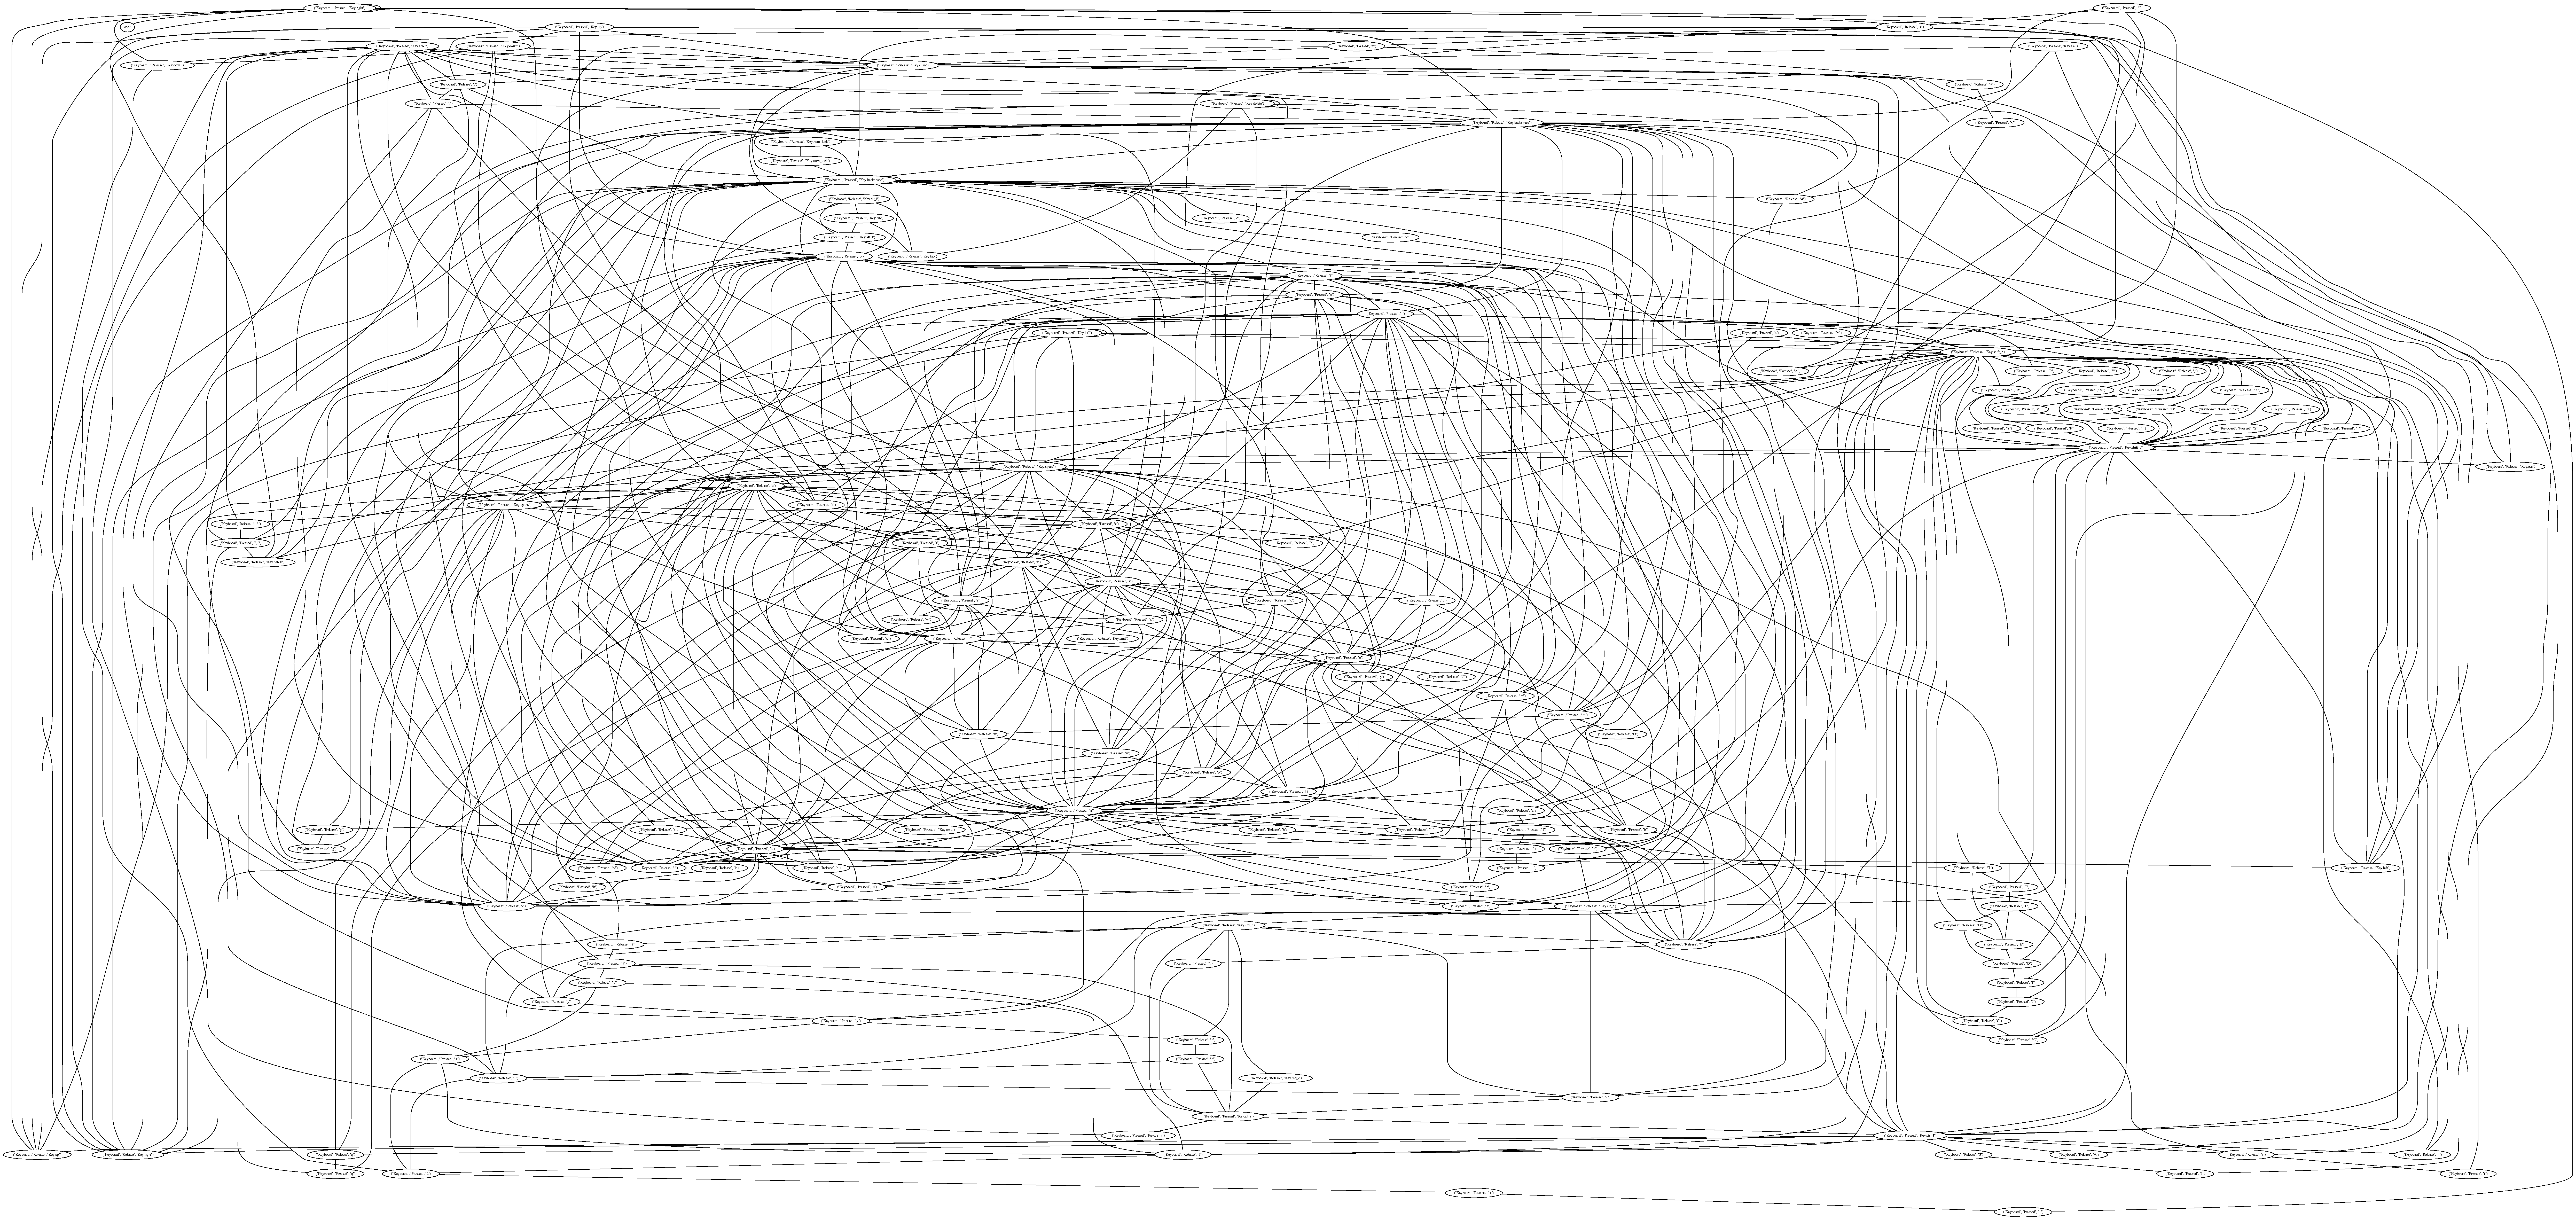
\includegraphics[width=1.0 \columnwidth]{Imagenes/GraphKB150.eps}
\caption{Grafo generado por el sujeto \emph{n\'umero 3} solo con acciones del 
 teclado.}
\label{fig:graphKB}
\end{figure}
\end{frame}


\begin{frame}
\begin{figure}[h]
\centering
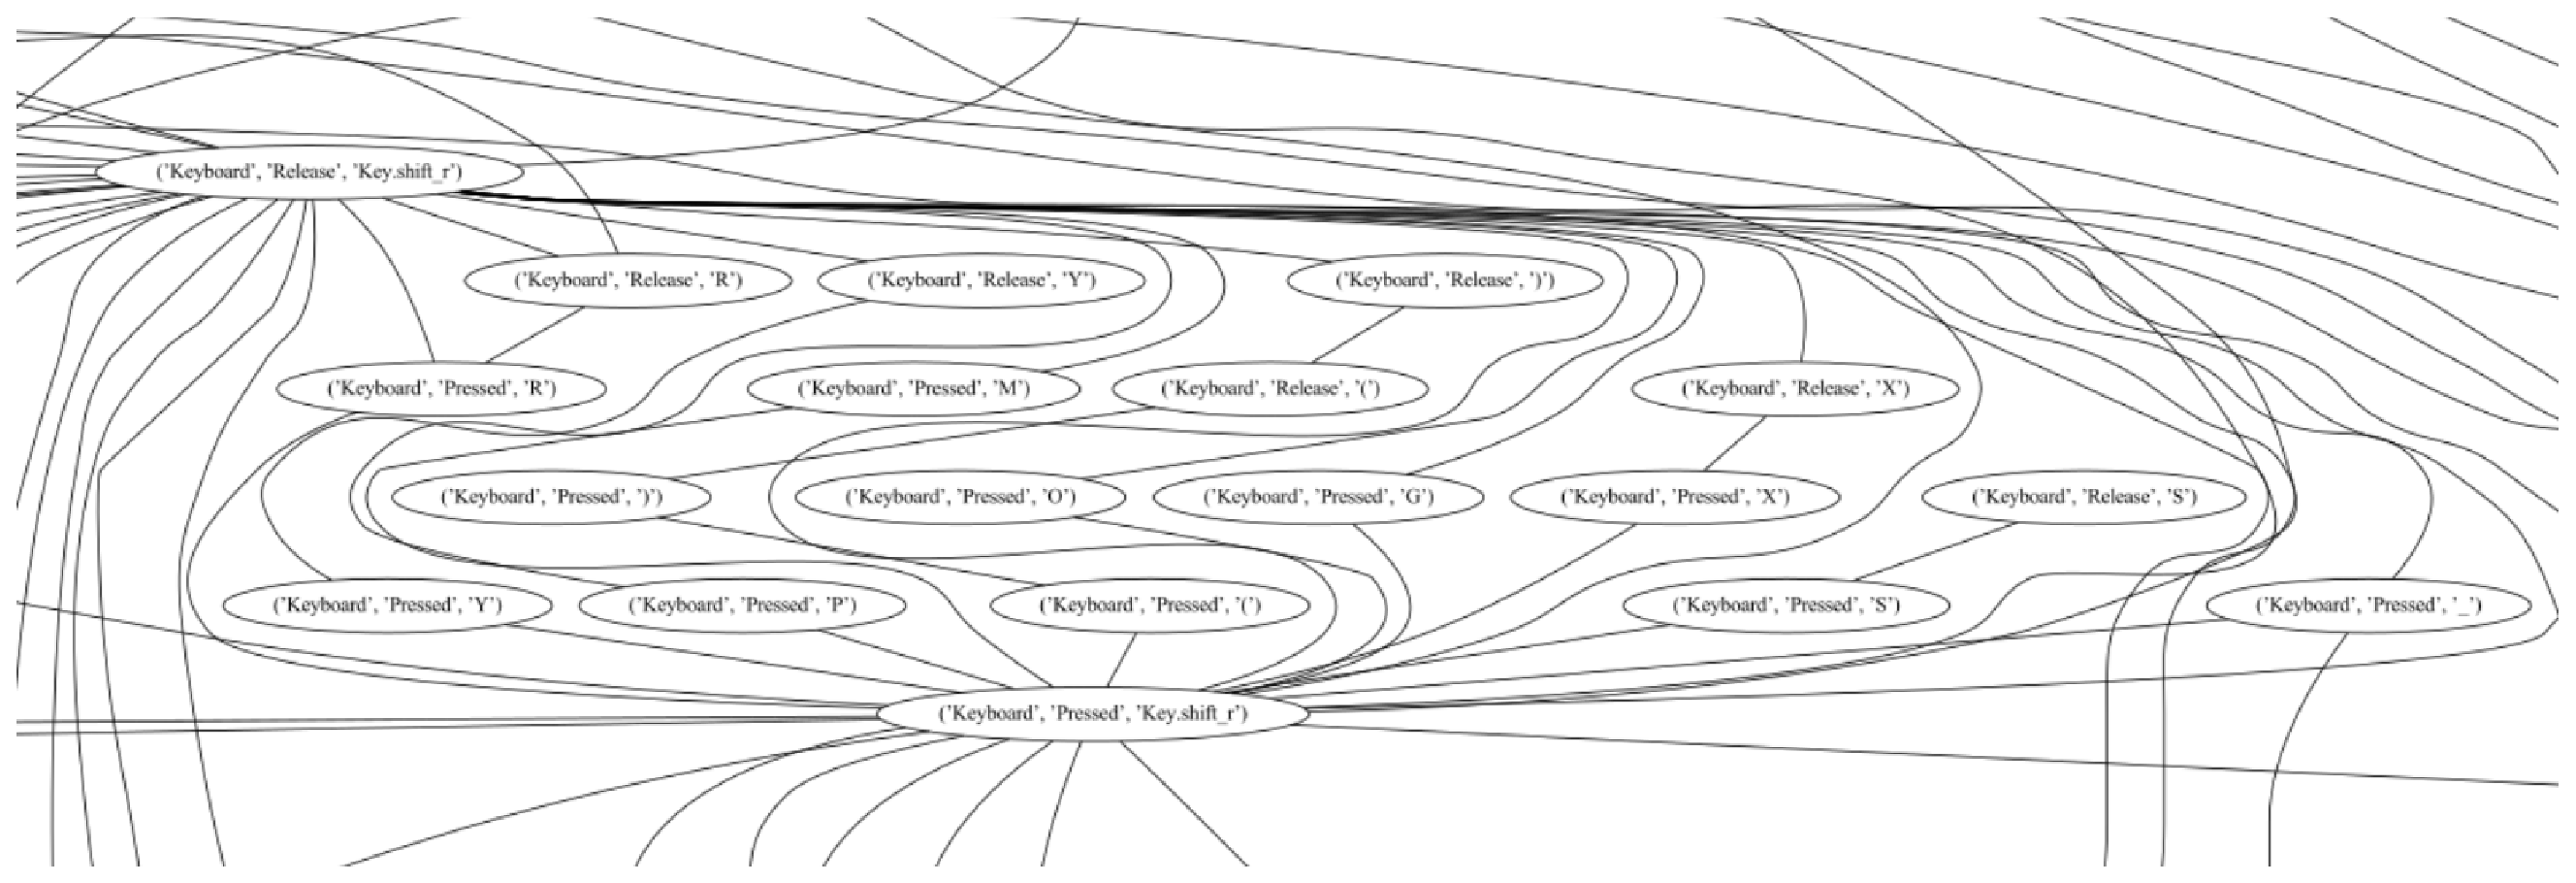
\includegraphics[width=1.0 \columnwidth]{Imagenes/ZoomKB150.eps}
\caption{Ampliaci\'on al grafo generado por el sujeto \emph{n\'umero 3} solo 
 con acciones del teclado.}
\label{fig:zoomKB}
\end{figure}
\end{frame}


\begin{frame}
\begin{figure}[h]
\centering
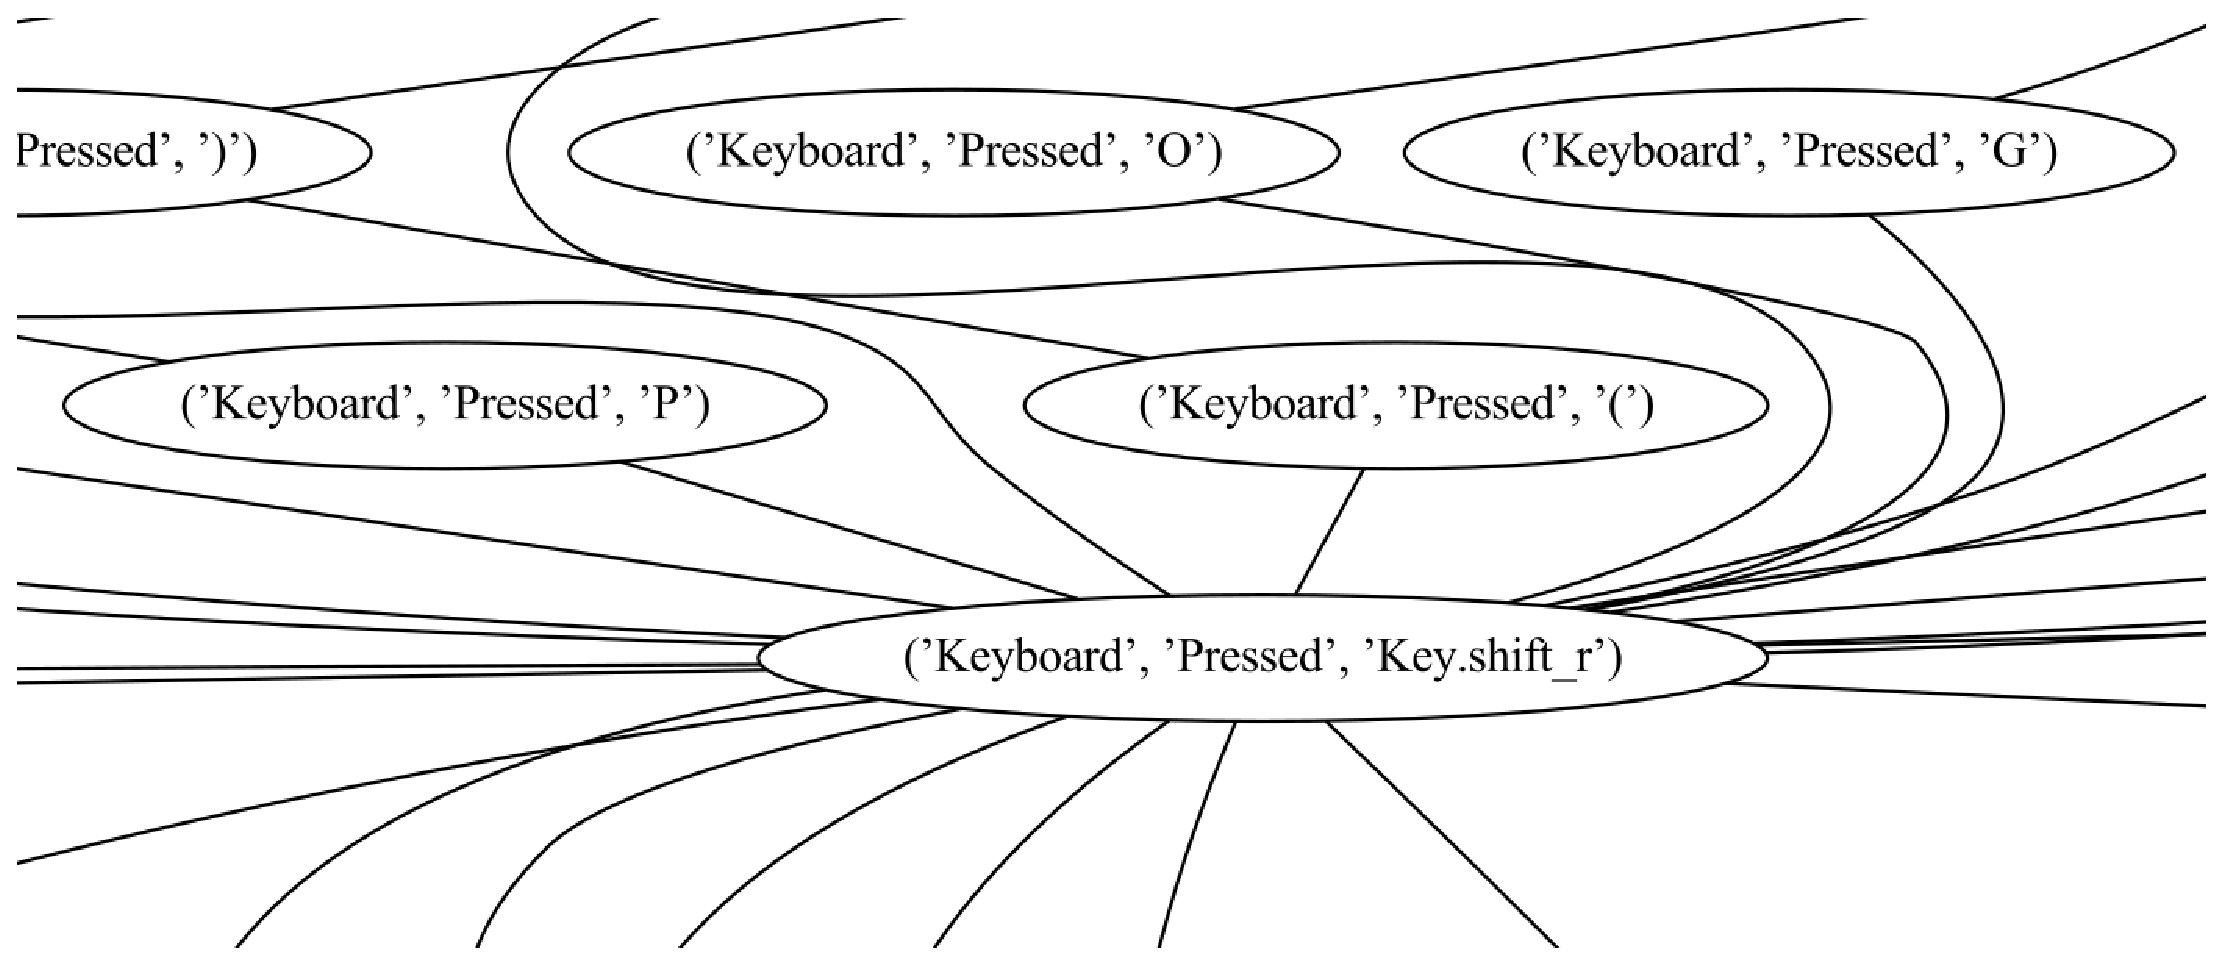
\includegraphics[width=1.0 \columnwidth]{Imagenes/MoreZKB150.eps}
\caption{Ampliaci\'on para la correcta visualizaci\'on de los nodos en el
 grafo generado por el sujeto \emph{n\'umero 3} solo con acciones del
 teclado.}
\label{fig:morezKB}
\end{figure}
\end{frame}

\begin{frame}
\frametitle{Resultados}

\begin{block}{Condiciones:}
\begin{columns}[T]
\begin{column}{.5\textwidth}
\begin{itemize}
\item {70 incidencias en el nodo}
\item {5 repeticiones de la secuencia}
\end{itemize}
\end{column}

\begin{column}{.5\textwidth}
\begin{itemize}
\item {No \textbf{empezar} con \emph{``Release''}}
\item {No \textbf{terminar} con \emph{``Pressed''}}
\end{itemize}
\end{column}
\end{columns}
\end{block}
%\vspace{-0.5cm}

\begin{table}[]
\centering

\scalebox{0.8}{
\begin{tabular}{cccc}
\hline
\textbf{No. de }	
&	\textbf{Secuencias }	
&   \textbf{Secuencias }	
&	\textbf{Porcentaje de }	\\

\textbf{Sujeto}
&	\textbf{Aceptables}
&	\textbf{Totales}
&	\textbf{Precisi\'on}
	\\ \hline

1				
&	189						
&	525						
&	36.00 \%		\\

2				
&	165						
&	487						
&	33.88 \%		\\

3
&	151
&	467
&	32.33 \%		\\

4
&	56
&	180
&	31.11 \%		\\

5
&	55
&	155
&	35.48 \%		\\

6
&	43
&	151
&	28.47 \%		\\

7
&	66
&	205
&	32.19 \%		\\

\hline
\end{tabular}
}
\caption{Resultados con secuencias de una longitud m\'inima de 
 1 acci\'on.}
\label{tableRes1}
\end{table}

\end{frame}


\begin{frame}
\frametitle{Resultados}


\begin{table}[]
\centering

\scalebox{0.8}{
\begin{tabular}{cccc}
\hline
\textbf{No. de }	
&	\textbf{Secuencias }	
&   \textbf{Secuencias }	
&	\textbf{Porcentaje de }	\\

\textbf{Sujeto}
&	\textbf{Aceptables}
&	\textbf{Totales}
&	\textbf{Precisi\'on}
	\\ \hline

1
&	179
&	410
&	43.65 \%		\\
	
2
&	170
&	377
&	45.09 \%		\\

3
&	154
&	346
&	44.50 \%		\\

4
&	52
&	119
&	43.69 \%		\\

5
&	49
&	108
&	45.37 \%		\\

6
&	38
&	78
&	48.71 \%		\\

7
&	60
&	145
&	41.37 \%		\\
\hline
\end{tabular}
}
\caption{Resultados con secuencias de una longitud m\'inima de 
 2 acciones.}
\label{tableRes2}
\end{table}
\end{frame}

\begin{frame}
\frametitle{Resultados}

\begin{columns}[T]
		\begin{column}{.33\textwidth}
			\begin{block}{\small{Es la palabra ``el''}}
				\centering
				Keyboard,Pressed,e	\\
				Keyboard,Release,e	\\
				Keyboard,Pressed,l	\\
				Keyboard,Release,l	\\
			\end{block}
		\end{column}

		\begin{column}{.33\textwidth}
			\begin{block}{\small{ La tarea es utilizada en el software
			 Blender para girar el objeto en el eje Y}}
				\centering
				Keyboard,Pressed,G\\
				Keyboard,Release,G\\
				Keyboard,Pressed,Y\\
				Keyboard,Release,Y\\
			\end{block}
		\end{column}
		
		\begin{column}{.33\textwidth}
			\begin{block}{\small{En Windows es utilizada esta combinaci\'on
			 de teclas para cambiar entre las ventanas abiertas.}}	
				\centering
				Keyboard,Pressed,alt\_l	\\
				Keyboard,Pressed,tab	\\
				Keyboard,Release,tab	\\
				Keyboard,Release,alt\_l	\\
			\end{block}
		\end{column}
		
	\end{columns}
\end{frame}


\subsection{Discusi\'on}
\begin{frame}
\frametitle{Discusi\'on}

\begin{table}[h]
\centering
\scalebox{0.9}{
\begin{tabular}{m{5cm}|m{5cm}}
\hline
\textbf{Creador de macros}
&
\textbf{Software desarrollado} \\
\hline
Hay que indicar manualmente cuando empieza y termina la acci\'on deseada	
 &	
Se monitorea cada acci\'on realizada por el usuario.\\
\hline

El usuario graba manualmente la tarea que desea automatizar	
 &
Se muestra al usuario las acciones que realiza con mayor frecuencia para que
  \'el decida cual guardar\\
\hline

El usuario requiere conocimiento del software para crear tareas complejas 	
 &
El usuario no requiere editar las tareas\\
\hline
\end{tabular}
}
\caption{An\'alisis comparativo del software con un generador de macros.}
\label{vsmacros}
\end{table}

\end{frame}


\begin{frame}
\frametitle{Discusi\'on}

\begin{table}[h]
\centering
\scalebox{0.9}{
\begin{tabular}{m{5cm}|m{5cm}}
\hline
\textbf{Robotic Process Automation}
&
\textbf{Software desarrollado} \\

\hline
Hay que indicar manualmente cuando empieza y termina la acci\'on deseada.
&
Se monitorea cada acci\'on realizada por el usuario.\\

\hline
Por medio de t\'ecnicas de reconocimiento de im\'agenes y monitoreo a los
 dispositivos de E/S, se determina la acci\'on realizada y el momento de 
 ejecuci\'on. 
&
Por medio del an\'alisis en tiempo ejecuci\'on de un grafo dirigido se 
 obtienen las tareas realizadas.\\

\hline
Se automatiza un proceso en espec\'ifico.
&
Se automatiza la tarea que m\'as realice el usuario.\\

\hline
\end{tabular}
}
\caption{An\'alisis comparativo de la propuesta con Robotic Process
 Automation.}
\label{vsrpa}
\end{table}

\end{frame}